%
\begin{enumerate}[label=\thesubsection.\arabic*.,ref=\thesubsection.\theenumi]
\item  In  
	\figref{fig:tri_icentre}, the bisectors of $\angle B$ and $\angle C$	 meet at $\vec{I}$.
Show that $IA$ bisects $\angle A$.
\begin{figure}[!ht]
	\begin{center}
		
		{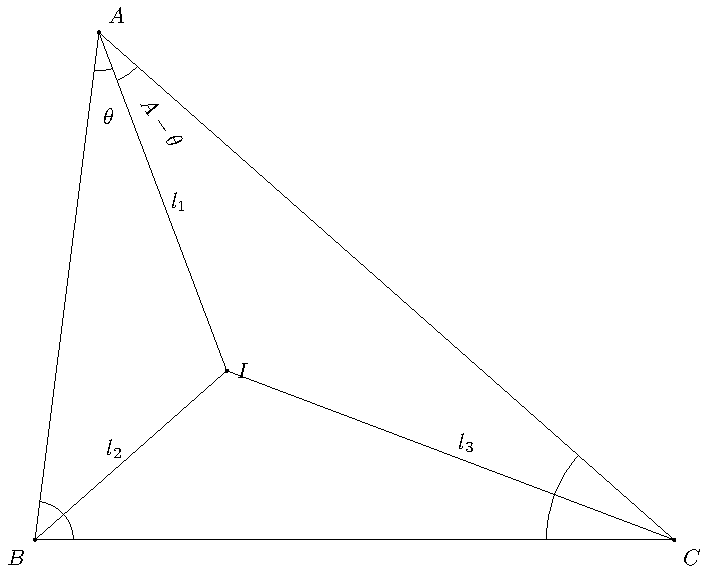
\includegraphics[width=0.6\columnwidth]{figs/trig_id/angbis/tri-icentre.pdf}}
	\end{center}
	\caption{Incentre $I$ of $\triangle ABC$}
	\label{fig:tri_icentre}	
\end{figure}
\\
\solution
Using sine formula
in
\eqref{eq:tri_sin_form}
  \begin{align}
  \frac{l_1}{\sin\frac{C}{2}}
  = 
   \frac{l_3}{\sin \brak{A-\theta}}
  ,\
   \frac{l_3}{\sin\frac{B}{2}}
=\frac{l_2}{\sin\frac{C}{2}}
  ,\
\frac{l_2}{\sin \theta}
	  =
  \frac{l_1}{\sin\frac{B}{2}}
  \end{align}
  Multiplying the above equations, 
  \begin{align}
  \sin \theta &= \sin \brak{A - \theta}
  \\
	  \implies \theta &=A - \theta 
	  \text{ or, } \theta = \frac{A}{2}
  \end{align}
  \item 
	\figref{fig:tri_iradius}, 
	is obtained from 
	\figref{fig:tri_icentre}	
	with
  \begin{align}
	  ID \perp BC, \, 
	  IE \perp AC, \, 
	  IF \perp AB.
  \end{align}
  Show that 
  \begin{align}
	  ID=   
	  IE= 
	  IF=r 
	\label{eq:tri_iradius}	
  \end{align}
		\begin{figure}[!ht]
	\begin{center}
		{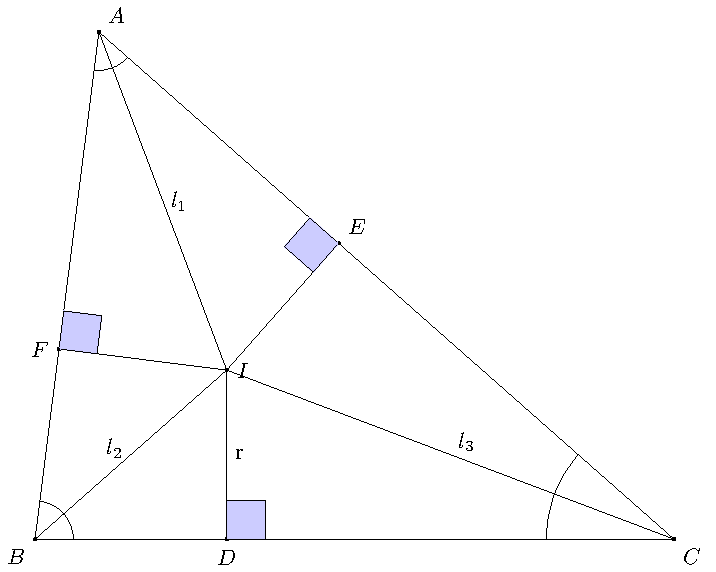
\includegraphics[width=0.6\columnwidth]{figs/trig_id/angbis/tri-iradius.pdf}}
	\end{center}
	\caption{Inradius $r$ of $\triangle ABC$}
	\label{fig:tri_iradius}	
\end{figure}
		\solution
In $\triangle$s $IDC$ and $IEC$, 
		\begin{align}
ID = IE=  \frac{l_3}{\sin\frac{C}{2}}
		\end{align}
		Similarly, 
in $\triangle$s $IEA$ and $IFA$, 
		\begin{align}
IF = IE=  \frac{l_1}{\sin\frac{A}{2}}
		\end{align}
		yielding 
	\eqref{eq:tri_iradius}	
  \item In
	\figref{fig:tri_iradius}, show that
  \begin{align}
	  BD=BF ,\, 
	  AE=AF ,\, 
	  CD=CE 
  \end{align}
  \solution  From 
\figref{fig:tri_iradius}, in $\triangle$s $IBD$ and $IBF$, 
		\begin{align}
			x = BD = BF = r \cot \frac{B}{2}
		\end{align}
		Similarly, other results can be obtained.
\item The circle with centre $\vec{I}$ and radius $r$ in  
	\figref{fig:tri_icircle}	
is known as the {\em incircle}. 
\begin{figure}[!ht]
	\begin{center}
		{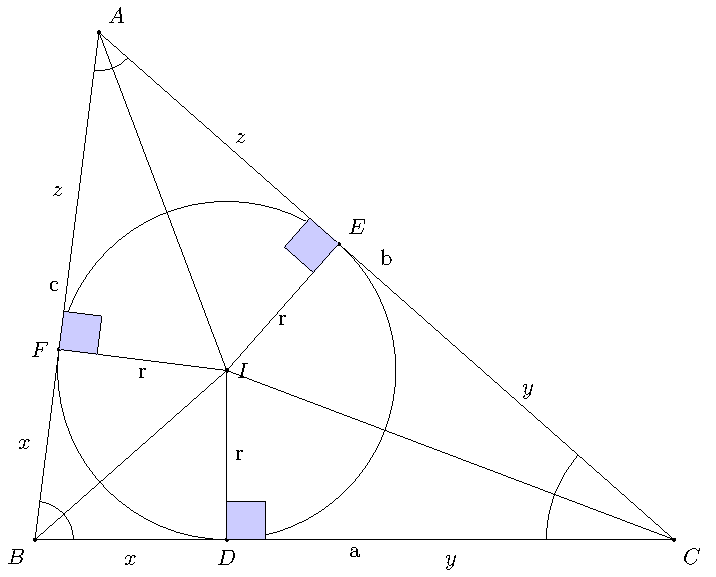
\includegraphics[width=0.6\columnwidth]{figs/trig_id/angbis/tri_icircle.pdf}}
	\end{center}
	\caption{Incircle of $\triangle ABC$}
	\label{fig:tri_icircle}	
\end{figure}
\item The lengths of tangents drawn from an external point to a circle are equal.
\item In an isosceles $\triangle ABC$, with $AB = AC$, $BE$ and $CF$ are the bisectors of $\angle B$ and $\angle C$ respectively.   Show that 
\begin{align}
BE = CF
	\label{eq:tri_isoc_ang_bsect}
\end{align}
\begin{figure}[H]
	\centering
		{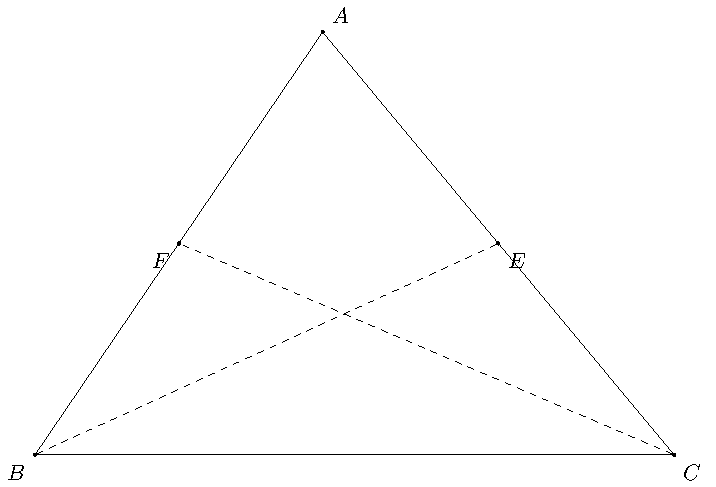
\includegraphics[width=0.6\columnwidth]{figs/trig_id/angbis/tri_isoc_ang_bsect.pdf}}
	\caption{}
	\label{fig:tri_isoc_ang_bsect}
\end{figure}
\solution
%
In $\triangle$ s $BEC$ and $BFC$, using the sine formula, 
\begin{align}
	\label{eq:tri_isoc_ang_bsect-inter}
\begin{split}
	\frac{BE}{\sin C}
	&=\frac{BC}{\sin \brak{\frac{B}{2}+C}}
	\\
	\frac{CF}{\sin B}
	&=\frac{BC}{\sin \brak{\frac{C}{2}+B}}
\end{split}
\end{align}
$\because B = C$, from the above, we obtain
	\eqref{eq:tri_isoc_ang_bsect}.
\item Show that
\begin{align}
\sin 5\theta &= 5\sin \theta - 20\sin^3 \theta \cos^2 \theta + 16\sin^5 \theta \\
\sin 3\theta &= 3\sin \theta - 4\sin^3 \theta
\label{eq:sin3-5}
\end{align}
\item 
	In \figref{fig:tri_isoc_ang_bsect}, if $BE = CF$, show that the triangle is isosceles.
	\\
	\solution
	From \eqref{eq:tri_isoc_ang_bsect-inter},
\begin{align}
	\sin C
\sin \brak{\frac{C}{2}+B}
	&=
\sin \brak{\frac{B}{2}+C}
\sin B
\\
	\implies 2\sin C
\sin \brak{\frac{C}{2}+B}
	&=
2\sin B
\sin \brak{\frac{B}{2}+C}
\\
\cos \brak{B - \frac{C}{2}}
-\cos \brak{B + \frac{3C}{2}}
	&=
\cos \brak{C - \frac{B}{2}}
-\cos \brak{C + \frac{3B}{2}}
\end{align}
using \eqref{eq:trig_id_sum_diff4},
which can be expressed as
\begin{align}
\cos \brak{C - \frac{B}{2}}
-
\cos \brak{B - \frac{C}{2}}
-\cos \brak{C + \frac{3B}{2}}
+
	\cos \brak{B + \frac{3C}{2}}
	=0
\end{align}
which, using \eqref{eq:trig_id_sum_diff4},
yields
\begin{align}
 2\sin \brak{ \frac{B +C}{2}}
	\sin \sbrak{ \frac{3\brak{B -C}}{2}}
	+ 2\sin \sbrak{ 5\frac{\brak{B +C}}{2}}
	\sin \sbrak{ \frac{\brak{B -C}}{2}}
	=0
\label{eq:bisect-conv}
\end{align}
Let
\begin{align}
	\theta = \frac{B -C}{2},\
	\alpha= \frac{B +C}{2}
\end{align}
Substituting the above in 
\eqref{eq:bisect-conv},
\begin{align}
 \sin \alpha \sin 3\theta
	+ \sin 5 \alpha \sin \theta = 0
\label{eq:bisect-conv-at}
\end{align}
Substituting
from \eqref{eq:sin3-5}
in \eqref{eq:bisect-conv-at} and simplifying,
\begin{align}
 \sin \alpha \sin \theta
	\brak{3- 4\sin^2 \theta + 5- 20\sin^2 \alpha \cos^2 \alpha + 16\sin^4\alpha } = 0
%\label{eq:bisect-conv-at}
\end{align}
One possible solution of the above equation is
\begin{align}
	3- 4\sin^2 \theta + 5- 20\sin^2 \alpha \cos^2 \alpha + 16\sin^4\alpha  = 0
	\\
	4- 4\sin^2 \theta + 4- 20\sin^2 \alpha \brak{1-\sin^2 \alpha} + 16\sin^4\alpha  = 0
\end{align}
which, upon 
substituting from 
\eqref{eq:tri_sin_cos_id}
results in 
\begin{align}
	\cos^2 \theta + 1- 5\sin^2 \alpha  +36 \sin^4\alpha  = 0
	\\
	=
	\cos^2 \theta + \brak{1- 6\sin^2 \alpha}^2  + 7\sin^2\alpha  = 0
\end{align}
For the above equation to have a solution, 
\begin{align}
	\cos \theta = 0, \sin^2\alpha = \frac{1}{6}, \sin \alpha = 0. 
\end{align}
which is impossible.  Another possible solution is 
\begin{align}
	\sin \alpha = \sin \frac{B+C}{2} = 0
	\\
	\implies \cos \frac{A}{2} = 0, \text{ or, }
	A = \pi, 
\end{align}
which is impossible.  Hence, the only possible solution is
\begin{align}
	\sin \theta = \sin \frac{B-C}{2} = 0
	\\
	\implies \frac{B-C}{2} =0, \text{ or, }
	B = C.
\end{align}
\end{enumerate}
